\documentclass[a4paper, 11pt]{article}
\usepackage[utf8]{inputenc}
\usepackage[T1]{fontenc}
\usepackage[french]{babel}
\usepackage{hyperref}
\usepackage{wrapfig}
\usepackage{fancyhdr}
\usepackage{graphicx}
\usepackage{titling}
\usepackage{sectsty} %% taille des textes
\usepackage{tocloft}%% taille table des matières
\usepackage{tabto}
\usepackage{etoolbox}
\usepackage{subcaption}
 
\pagestyle{fancy}
\fancyhf{}

%% Tête et pied de page
\lhead{SAFExTY}
\rfoot{Page \thepage}
\lfoot{Janvier 2020}

%% Configuration des sections
\sectionfont{\LARGE}
\subsectionfont{\Large}
\renewcommand\cftsecfont{\Large\bf}
\renewcommand\cftsubsecfont{\large}
\renewcommand\cftsecafterpnum{\par\addvspace{10pt}}


%% Pré-titre
\pretitle{
  \begin{center}
  
\includegraphics[width=7cm]{images/SAFExTY-Text.png}\\
}

%% Titre
\title{\Huge Cahier des charges}
\date{Janvier 2020}

\posttitle{\end{center}}

\begin{document}

%% Page de titre
\maketitle
\pagebreak

%% Page table des matières
\begingroup
  \flushbottom
  \setlength{\parskip}{0pt plus 1fil}%
  \renewcommand{\contentsname}{\huge\textsc{Table des matières\newline}}
  \tableofcontents
  \newpage
\endgroup

%% Les autres pages
\section{Introduction}

Depuis 10 ans, le nombre d'interventions de secours à personne augmente de 8 à 10\% chaque année. Pour continuer à répondre aux demandes en temps acceptable, les services de secours ont migré, il y a quelques années, vers des systèmes informatisés de gestion des interventions, des équipements et du personnel. Cela a permis à chaque agent de pouvoir gérer sa disponibilité pour pouvoir partir en intervention à la demande, de commander ou échanger du matériel, de se former et de communiquer en temps réel. Cependant, ces systèmes sont anciens et l’ensemble forment un assemblage de briques bien séparées qui rend leurs utilisations complexes et peu efficaces. \\

C’est pourquoi, en collaboration avec la caserne des Sapeurs-Pompiers de Saint-Georges-D’espéranche (dans le nord-isère), nous allons réaliser un projet qui répond à des besoins spécifiques de centralisation et de gestions des agents et équipements, sans remplacer l'existant, tout en accentuant la sécurité des systèmes. \\

Le projet se découpe en quatre grandes parties :
\begin{itemize}
  \item \textbf{Gestion du personnel :} obtenir et maintenir à jour automatiquement toutes les informations sur le personnel (nom, grade, visites médicales, formations réalisées, nombre d'interventions, suivi des formations, équipements...) et communiquer avec la caserne (annonces écrites, messages programmés...)\\
  \item \textbf{Gestion du matériel et véhicules :} obtenir et maintenir à jour automatiquement les réserves matérielles (expiration des consommables, suivi de la consommation, commandes automatiques, prévisions...) et des véhicules (nombre d'interventions, fiche d'inventaire modifiable, signalement de pannes/problèmes, rappel contrôle technique...)\\
  \item \textbf{Formation et regroupement des ressources :} centraliser l'ensemble des documents de formations et proposer un support interactif d’entraînement, d'apprentissage et de formations (recherche de référentiels, de techniques, préparation aux formations, cours en ligne avec évaluations indicatives, mises en situation, QCMs...)\\
  \item \textbf{Adaptation et sécurité : } se baser sur les technologies existantes utilisées par le SDIS\footnote{Service Départemental d'Incendie et de Secours : service publique en charge des sapeurs-pompiers} tout en assurant de bout en bout le secret professionnel, la confidentialité et l'intégrité de chaque informations (stockage et communication entre clients-serveurs sécurisés).
\end{itemize}
\section{L'équipe}
\subsection{La formation du groupe}

Voulant un projet autre qu'un jeu-vidéo et qui puisse être utile à quelqu’un, nous avons décidé de nous regrouper sur SAFExTY : une plateforme de gestions et de formations sécurisées pour les sapeurs-pompiers.

\subsubsection{Jean BARBAROUX}
Jean est un élève dévoué qui prend son rôle de chef de projet très à cœur. De ce fait, et de par son expérience, il est prêt à chéffer de façon exemplaire en étant un élève moteur pour son groupe tout en étant un soutien psychologique. Il est également le plus âgé de son groupe, et sûrement l'un des plus âgés de la promo !

\subsubsection{Valentin CHASSIGNOL}
Valentin est sapeur-pompier volontaire depuis 2018 mais aussi un grand amateur du monde numérique. Il est passionné par l'informatique et le sport. Ce projet va lui permettre de mettre en pratique ses acquis et de découvrir de nouvelles technologies. Dévoué, il souhaite lier deux de ses passions. Grâce à son expérience, Valentin agira sur tous les fronts et là où on a besoin de lui. Il est déterminé à mener se projet à bien, même s'il doit sacrifier quelques heures de sommeil !

\subsubsection{Annabelle CHEVREAU}
Depuis sa découverte de l'informatique et plus précisément de la programmation en classe de première SSI, Annabelle est déterminée à accroître ses connaissances. En classe de Terminale S, elle a choisi l'option ISN qui lui a permis d'apprendre le C et de réaliser des petits projets dont un jeu en 2D, avec un langage appris de façon autodidacte. Déterminée, elle participera du mieux possible à la bonne réussite du projet.

\subsubsection{Florian DREVET}
Florian, en plus de l'informatique, aime jouer aux échecs et participer à des événements sportifs. Faisant partie de plusieurs associations, il est motivé par la création d'un logiciel. Ce projet va lui permettre d'acquérir de nouvelles connaissances en informatique et sur le travail de groupe. Enjoué à l'idée d'une collaboration avec les sapeurs-pompiers, il espère pouvoir les aider dans leurs tâches. Le groupe pourra compter sans détour sur son investissement ! Créatif, il sera source d'inspiration afin de mener le projet à son terme !

\section{Le cœur projet}

\subsection{Introduction du projet}
\subsubsection{Origine du projet}
Nous nous sommes réunis dans ce groupe car nous voulions créer un logiciel pouvant aider une caserne de pompiers. Cependant devant l'impossibilité de réaliser ce projet nous sommes resté sur l'idée des secours : nous sommes par la suite partie sur un jeu vidéo de gestion des services de secours d'une ville afin de ne pas être totalement dé-paysagés.

\subsubsection{Nature du projet}
Nous allons travailler à la création d'un jeu vidéo qui puisse être jouée par le plus grand nombre. Sa visée principale est d'apprendre à gérer la construction d'une ville et principalement de son service de secours. Le joueur devra faire évoluer sa ville en améliorant les bâtiments et le pôle de secours. Afin de permettre ces améliorations, le joueur devra gagner des points en réalisant des interventions sur différents incidents présents dans la ville, tel qu'un accident de voiture, un incendie....

\subsection{Objet de l'étude}

\subsubsection{Les attentes et objectifs}
La création d'un jeu vidéo demande des connaissances dans divers domaines. De plus, travailler en groupe va nous demander d'organiser et de savoir déléguer le travail afin de se concentrer sur une seule partie et d'avoir confiance en nos coéquipiers. Chaque partie devant à terme pouvoir être fonctionnelle et accessible pour tous ! L'organisation du code, les noms des classes, des fonctions doivent être claires et suffisamment documentés. Le code doit être également lisible, clair et compris de tous afin que le groupe puisse aisément le modifier et l'adapter en fonction des besoins de chacun et des éventuels problèmes qui pourraient survenir de façon inopinée.

\subsubsection{Définition du projet}
 Nous souhaitons donc réaliser un jeu sur la gestion d'une ville, et de son service de secours. Il se découperait en plusieurs parties:\\
    \begin{itemize}
        \item \textbf{Gestion de la map} :\\
        Dans cette partie il faudra définir la map sur laquelle reposera le jeu, c'est-à-dire là où les bâtiments peuvent être construits ainsi que la place nécessaire sur les cases de jeu qu'ils représentent. La Map sera en vue 2D isométrique, c'est un bon moyen de simuler de la 3D sans ses contraintes (voir annexes). La carte sera composée de différents reliefs : plaines, montagnes, rivières. Seront également présents des éléments naturels tels que des arbres, des buissons, des rochers, des fleurs. Ces objets pourront être détruits afin de libérer de l'espace constructible. Il faut alors pouvoir positionner les bâtiments, les construire, les déplacer et les détruire, chaque action prenant un certain temps.\\
        
        \item \textbf{Gestion des bâtiments} :\\
        Ici, il faudra créer les bâtiments et les définir. Il faudra donc exprimer les caractéristiques de chaque bâtiment dont on peut déjà lister une partie :
        \begin{itemize}
            \item la taille qu'il prend sur la map (zone nécessaire à sa construction)
            \item le coût en ressource (temps et argent) pour sa construction
            \item le temps de construction
            \item le coût d'une amélioration
            \item le temps d'une amélioration
            \item ce que rapporte le bâtiment (en fonction du niveau)
            \item ce qu'il débloque (en action, bâtiment...)
        \end{itemize}
        Le tout avec différentes textures bien évidemment.\\

        \item \textbf{Gestion des incidents} :\\
        Cette partie correspond à gérer les différents incidents qui seront présents dans le jeu en fonction du nombre d'habitants, du niveau de développement de la ville, du niveau du pôle de secours... Les incidents pourront aller de la simple petite blessure/coupure à un gros accident de voiture ou incendie sur lesquels les secours pourront/devront se rendre, dépendamment des ressources disponibles (voitures, camions, support aérien.), plus ou moins rapidement.
        \\
    
        \item \textbf{Stockage Réseau, Sauvegarde \& Launcher}:\\
        Le joueur a une progression liée à son compte. Il doit alors depuis le site web (ou le jeu) pouvoir se créer un compte qui permettra de synchroniser sa partie, de connaître ses statistiques pour un éventuel leader board sur le site internet.
        
        Le Launcher doit permettre de charger les données du joueur dans le jeu et se charger de synchroniser chaque sauvegarde. Il sera réalisé grâce à Qt Sharp (dérivé de QT accessible sur la plateforme .NET).
         \\
    \end{itemize}

\subsection{État de l'art}

La plupart des jeux du type city-builder (contruction et gestion d'une ville) pourraient ressembler à notre jeu.\\ 

Les jeux \textit{city ville\footnotemark[1]}, \textit{sim city\footnotemark[2]} se rapportent à l'univers de notre jeu puisqu'il faut construire et gérer une ville. Cependant ces jeux restent uniquement axés sur la gestion de la ville, là où notre jeu s'axe sur la ville mais également sur les services de secours. Il y a donc une double gestion.\\

Ce principe de double gestion se retrouve dans d'autres jeux : On peut citer le jeu \textit{township\footnotemark[3]} qui pourrait ressembler au but de notre jeu. Le jeu est basé sur la gestion d'une ville en liant la gestion d'une ferme. Dans notre jeu nous lions gestion d'une ville avec gestion des services de secours. Cependant nous allons ajouter plus d'interaction entre la ville et le poste de secours. Dans la ville se produira des accidents, des problèmes que le joueur devra résoudre à l'aide des services de secours.\\

Il y a également le jeu \textit{Airport city\footnotemark[4]} qui est le jeu qui doit se rapporter le plus à notre jeu. Il associe la gestion d'un aéroport et d'une ville. De plus les deux sont liés. Pour avoir plus de passagers il faut plus d'habitant dans la ville, ou pour avoir de l'énergie dans l'aéroport il faut des éoliennes, etc. Il faut donc très bien gérer la ville pour pouvoir permettre à son aéroport de grandir rapidement. Dans notre jeu les servies de secours évolueront en même temps que la ville. Plus le nombre d'habitants sera important et plus le nombre d'accidents augmentera.


\footnotetext[1]{Lien vers le descriptif du jeu city ville :
\url{https://www.jeuxonline.info/jeu/CityVille}} 
\footnotetext[2]{Lien vers le descriptif du jeu simcity sur le site EA : 
\url{https://www.microsoft.com/fr-fr/p/township/9nblggh3vrmz}}  
\footnotetext[3]{Lien vers le descriptif du jeu township sur le microsoft store :
\url{https://www.microsoft.com/fr-fr/p/township/9nblggh3vrmz}} 
\footnotetext[4]{Lien information du jeu dans le microsoft store : 
\url{https://www.microsoft.com/fr-fr/p/airport-city/9wzdncrfjchj}} 

\section{Organisation}
\subsection{Découpage de l'équipe}
Qui fait quoi, comment, avec qui/quoi...

\subsection{Répartitions des taches}

\subsection{Programme soutenance}
% Tout ce qui se rapporte au projet sans en faire partie
\section{Environnement}
\subsection{Le site web}
Qui, Quoi, comment ?

\subsection{Finance}
Acheter ? Gagner ? Qui gère

\subsection{Communication et tests}
% Tout ce qui se rapporte au projet sans en faire partie

\section{Conclusion}
En conclusion, ce projet, bien que débutant avec un peu de retard est sur de bons rails. Notre équipe est fortement motivée. Ainsi, nous avons de bons axes de travail et une division des tâches équilibrées qui nous permettront d'etre toujours à jour dans nos taches et d'avancer le plus vite possible afin de pouvoir tester notre jeu et de profiter de celui-ci dans les plus brefs délais.
 
\section{Annexes}


\begin{figure}[h]
    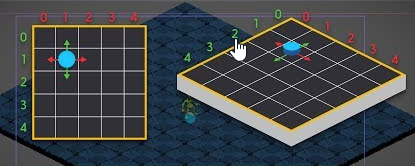
\includegraphics[height=5cm]{images/isovs.png} 
    \caption{Grille 2D avec vu isométrique}
    \label{fig:subim1}
\end{figure}

\begin{figure}[h]
 
\begin{subfigure}{0.5\textwidth}
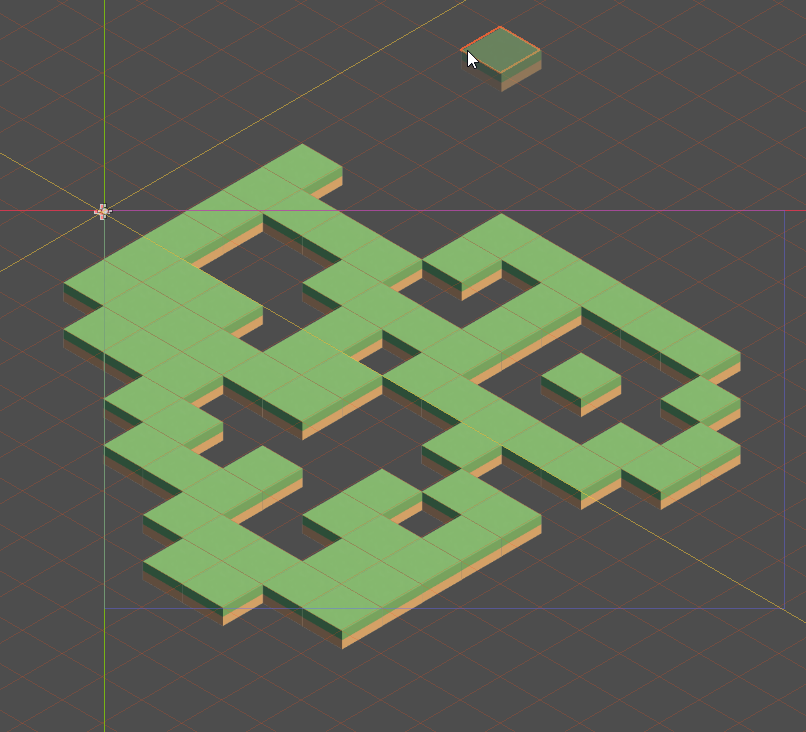
\includegraphics[width=0.9\linewidth, height=5cm]{images/2diso.png} 
\caption{Grille 2D avec vu isométrique}
\label{fig:subim1}
\end{subfigure}
\begin{subfigure}{0.5\textwidth}

\includegraphics[width=0.9\linewidth, height=5cm]{images/2diso2.png}
\caption{Exemple de rendu}
\label{fig:subim2}
\end{subfigure}
 
    \caption{Exemple de vue isométrique}
\label{fig:image2}
\end{figure}

\end{document}
